\chapter{Results {\&} Analysis}
\label{chap:resultsanalysis}

\section{Implementation that uses Simple Event Correlators own rule format (regex based)}
\todo{Why did we choose Go?}

\subsection{SEC rule format}



\begin{lstlisting}
type=single
ptype=regexp
pattern=(\S+)sshd.*
desc=This is a description
\end{lstlisting}

\subsubsection{type}
Type of rule. There are many different types here.
I have focused on rules using "SingleWithThreshold" which takes an action if there are X number of matches in Y time.

Single

Suppress

Calendar

SingleWithSuppress

Pair

PairWithWindow

SingleWith2Thresholds

EventGroup

SingleWithScript

Jump

\subsubsection{ptype}
Pattern type. RegExp is a Perl regular expression. Can use variables.

SubStr

PerlFunc

Cached

TValue

\subsubsection{pattern}
The pattern that the log line will we tested against. The value of this pattern is based on the ptype. For example, if the ptype is set to "RegExp", the pattern will be a Perl regular expression.

\subsubsection{desc}
Description field. But used for defining "scopes" when correlating.

\subsubsection{action}
The action to take when the rule "hits".

\subsubsection{continue}

\subsubsection{context}

\subsection{Implementation}
As discussed in chapter X, the programming language Go was chosen for implementing our new program to analyze our datasets. I have chosen to only implement the SingleWithTreshold type, and the RegExp pattern type (ptype). The "SingleWithTreshold" type triggers an action if there are X number of matches within Y time. We consider this to be the most usable rule type for our purpose. \com{What is the purpose?} For the pattern type, we choose to use "RegExp", which are Perl regular expressions. We consider this to be the best option for matching against syslog-based log lines.

Other than the fact that Go is a compiled language and Perl is a interpreted language, the main additions in our implementation is that our version:
\begin{itemize}
    \item Uses Go channels for re-injecting events into the context engine.
    \item The use of channels and goroutines gives us the ability to run in a threaded matter, utilizing multiple cores.
\end{itemize}

\subsubsection{Workers}
\todo{What are workers?}

\subsection{Results}
We want to see if our Go implementation can out-perform SEC when handling a high signal, low noise dataset. The following table shows the results for that:
\\
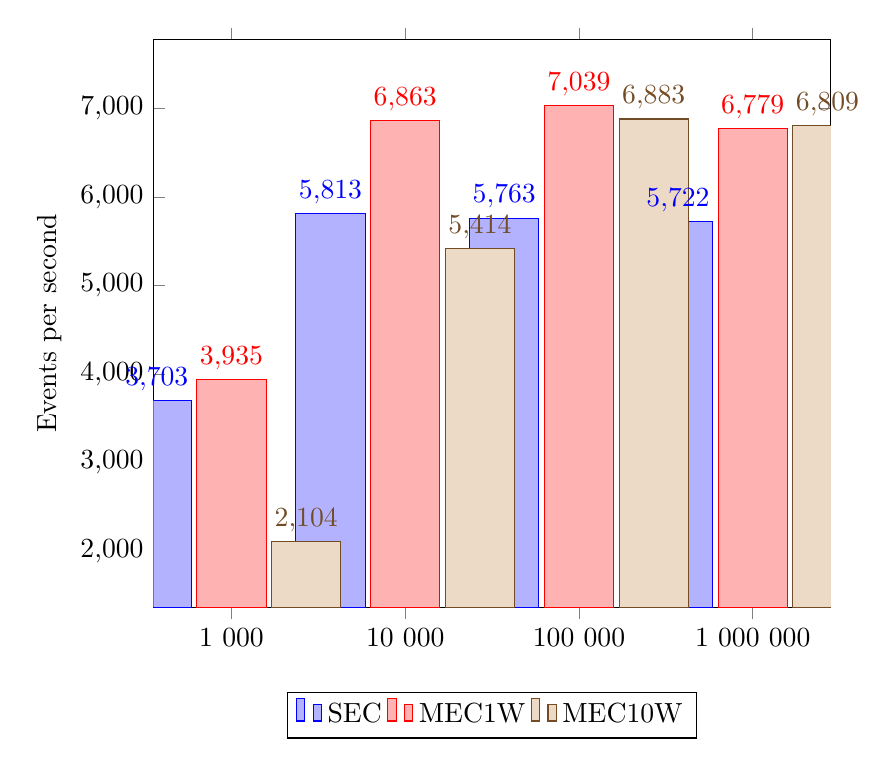
\begin{tikzpicture}
\begin{axis}[
    xtick=data,
	height=250pt,
	ylabel=Events per second,
	enlargelimits=0.15,
	legend style={at={(0.5,-0.15)},
	anchor=north,legend columns=-1},
	ybar,
	bar width=25pt,
	symbolic x coords={1 000, 10 000, 100 000, 1 000 000},
	nodes near coords,
	nodes near coords style={above}
]
\addplot coordinates {(1 000,3703) (10 000,5813) (100 000,5763) (1 000 000,5722)}; % SEC
\addplot coordinates {(1 000,3935) (10 000,6863) (100 000,7039) (1 000 000,6779)}; % MEC1W
\addplot coordinates {(1 000,2104) (10 000,5414) (100 000,6883) (1 000 000,6809)}; % MEC10W
\legend{SEC, MEC1W, MEC10W}
\end{axis}
\end{tikzpicture}
\\
These tests are run with 1 logical core on a "Intel(R) Core(TM) i7-7600U CPU @ 2.80GHz" (2 cores x 2 threads per core = max 4 logocal cores) and 24GB RAM.

\begin{itemize}
    \item Why is the MEC10W slower?
    \item Why are the runs on the 1 000 dataset generally lower?
\end{itemize}

By using all CPU cores available (4) instead of a single one, we can take better advantage of Gos concurrency model, and raise the throughput when using multiple workers and CPUs:

\pgfplotsset{scaled y ticks=false}
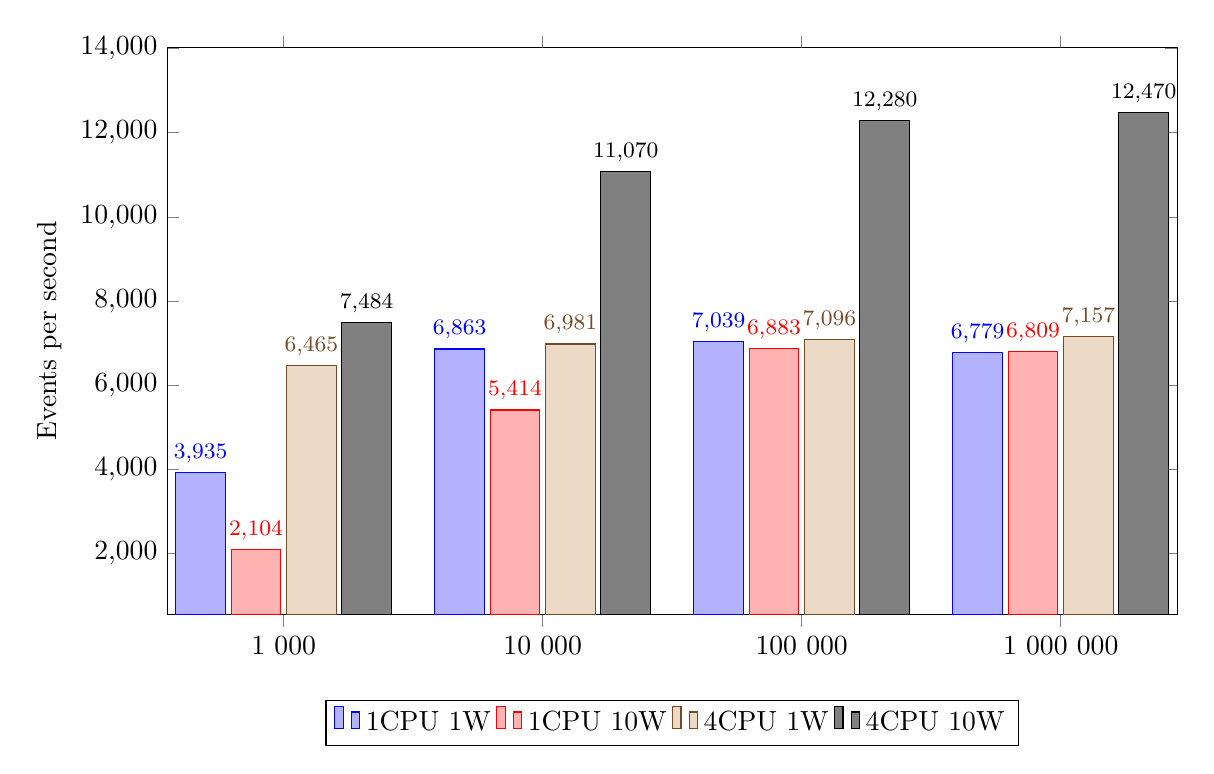
\begin{tikzpicture}
\begin{axis}[
    xtick=data,
    width=410pt,
	height=250pt,
	ylabel=Events per second,
	enlargelimits=0.15,
	legend style={at={(0.5,-0.15)},
	anchor=north,legend columns=-1},
	ybar,
	bar width=18pt,
	symbolic x coords={1 000, 10 000, 100 000, 1 000 000},
	nodes near coords,
	nodes near coords style={above, font=\footnotesize},
]
\addplot coordinates {(1 000,3935) (10 000,6863) (100 000,7039) (1 000 000,6779)}; % 1CPU 1W
\addplot coordinates {(1 000,2104) (10 000,5414) (100 000,6883) (1 000 000,6809)}; % 1CPU 10W
\addplot coordinates {(1 000,6465) (10 000,6981) (100 000,7096) (1 000 000,7157)}; % 4CPU 1W
\addplot coordinates {(1 000,7484) (10 000,11070) (100 000,12280) (1 000 000,12470)}; % 4CPU 10W
\legend{1CPU 1W , 1CPU 10W , 4CPU 1W , 4CPU 10W}
\end{axis}
\end{tikzpicture}

\begin{itemize}
\item Why is there a dip for 1CPU,10W when using a dataset of 1 000 events?
\item Why are the results of 1CPU,1W, 1CPU,10W and 10CPU,1W generally the same?
\item What can we say about 1CPU,10W "catching up" to the others around 100 000 events?
\end{itemize}

\todo{What are some further improvements to this? Outline why a new rule format could be better suited.}

\section{Implemented a new rule format}
This format relies less on the extensive use of Regexes \com{Hvorfor er dette en fordel? Hvorfor er dette valget smart? Beskriv dette i experiment delen?}, as we saw in the rules used by Simple Event Correlator. \todo{Elaborate on this}
\\
For each log line/event we:

\begin{enumerate}
    \item Tokenize the event into a Event struct. \com{Hva er dette?... Flytt beskrivelsen opp til Experiment i stedet?}
    \item Iterate over every rule, checking if the Event matches the detection-part of the rule.
    \begin{itemize}
        \item If there is a match, we run the Event through the context engine, to see if the conditions are met for the rule.
    \end{itemize}
\end{enumerate}

When we tokenize the event, we take a single line of log/event, and split it into its key-value representation. For instance, the following event log is a single line of text:
\begin{lstlisting}[breaklines=true]
<14>Feb 18 02:29:49 Client02.mrtn.lab Microsoft-Windows-Sysmon[2092]: Process Create:  RuleName:   UtcTime: 2020-02-18 10:29:49.839  ProcessGuid: {dadb16ad-bc9d-5e4b-0000-0010c8fd3600}  ProcessId: 1040  Image: C:\Windows\System32\whoami.exe  FileVersion: 10.0.17763.1 (WinBuild.160101.0800)  Description: whoami - displays logged on user information  Product: Microsoft Windows Operating System  Company: Microsoft Corporation  OriginalFileName: whoami.exe  CommandLine: whoami  CurrentDirectory: C:\Users\mrtn\  User: MRTNLAB\mrtn  LogonGuid: {dadb16ad-2c2d-5e17-0000-0020fc3c1b00}  LogonId: 0x1B3CFC  TerminalSessionId: 1  IntegrityLevel: Medium  Hashes: MD5=43C2D3293AD939241DF61B3630A9D3B6,SHA256=1D5491E3C468EE4B4EF6EDFF4BBC7D06EE83180F6F0B1576763EA2EFE049493A,IMPHASH=7FF0758B766F747CE57DFAC70743FB88  ParentProcessGuid: {dadb16ad-2cf1-5e17-0000-001027122b00}  ParentProcessId: 2748  ParentImage: C:\Users\mrtn\test.exe  ParentCommandLine: .\test.exe
\end{lstlisting}
But after tokenization, it looks like this:
\begin{lstlisting}[breaklines=true]
MachineName: Client02.mrtn.lab
ProcessType: Process Create: 
RuleName:   
UtcTime: 2020-02-18 10:29:49.839
ProcessGuid: {dadb16ad-bc9d-5e4b-0000-0010c8fd3600}
ProcessId: 1040
Image: C:\Windows\System32\whoami.exe
FileVersion: 10.0.17763.1 (WinBuild.160101.0800)
Description: whoami - displays logged on user information  Product: Microsoft Windows Operating System
Company: Microsoft Corporation 
OriginalFileName: whoami.exe
CommandLine: whoami
CurrentDirectory: C:\Users\mrtn\
User: MRTNLAB\mrtn
LogonGuid: {dadb16ad-2c2d-5e17-0000-0020fc3c1b00}
LogonId: 0x1B3CFC
TerminalSessionId: 1
IntegrityLevel: Medium
Hashes: MD5=43C2D3293AD939241DF61B3630A9D3B6,SHA256=1D5491E3C468EE4B4EF6EDFF4BBC7D06EE83180F6F0B1576763EA2EFE049493A,IMPHASH=7FF0758B766F747CE57DFAC70743FB88
ParentProcessGuid: {dadb16ad-2cf1-5e17-0000-001027122b00}
ParentProcessId: 2748
ParentImage: C:\Users\mrtn\test.exe
ParentCommandLine: .\test.exe
\end{lstlisting}
The tokenized version of the event log is stored as a Go struct, which makes it simpler to query specific parts of the event log directly, instead of having to parse the whole event log every time we want to access a single key-value pair. An example would be if we wanted to access the MachineName or CommandLine values from the above example, which would be done like this:  \lstinline{event['MachineName']} and \lstinline{event['CommandLine']}.


\subsection{Context}
\n{What is context?}
\\
When we want to do correlation between two or more events based on a rule, we need to have some kind of overview of what state our rule is in. When a new event arrives that triggers our rule, we need to know if this is the first event, if there are other events that have triggered before it, and most importantly, if the previous events that triggered the rule is within the given time frame of the rule. This is what we call "context".

\subsection{The Context Engine}
One of the benefits of our new implementation is the ability to process events concurrently. But when working with a context that is accessed by several workers concurrently, data races may appear. A data race occurs when two goroutines concurrently accesses the same variable (in this case the context variable), and at least one of the goroutines writes to the variable. The danger here is that we could have two or more goroutines with their own versions of the context that are out of sync. This could lead to data loss and/or a failure to detect when a rule-condition is met. The standard way of dealing with data races like this is to use a mutex. A mutex provides a locking mechanism to ensure that only one goroutine can manipulate a variable at a time.

In our implementation we have integrated a mutex in two different ways, using a shared context mutex and using a rule-based context mutex. \com{Det er ikke så interessant at vi har brukt to forskjellige, men hva oppnår vi? Hva var hensikten med dette?}

\subsubsection{Shared context}

For the shared context, we have a large map that looks like this:
\begin{lstlisting}
context := map[string]{
    Events  []Event
}
\end{lstlisting}
We access it by doing:
\begin{lstlisting}
c := context["CONTEXT_FOR_RULE_1"]
\end{lstlisting}
the variable \lstinline{c} now contain an array of \lstinline{event}s, if there are any for the given key \lstinline{CONTEXT_FOR_RULE_1}. In our implementation we use the ID of the rule for this lookup, as it is an (Universally unique identifier) UUID4-string, and is safe to use as a unique identifier.


Since we may both read and write to the \lstinline{c} variable, we need to lock a mutex for the \lstinline{context} map. We can do this like this:

\begin{lstlisting}
context := map[string]{
    Events  []Event
}
contextMutex := &sync.RWMutex{}

contextMutex.Lock()
c := context["CONTEXT_FOR_RULE_1"]

// Add or remove events to the context here

context["CONTEXT_FOR_RULE_1"] = c

contextMutex.Unlock()
\end{lstlisting}

We now have a goroutine-safe way of accessing and editing our context. The drawback of this is in the design, when multiple goroutines try to access the context, they will have to wait for their turn to lock on the context.

\subsubsection{Rule-based context}
For the rule-based context, both the context and the context mutex is defined in the rule struct itself:
\begin{lstlisting}
type context struct {
    events []event
}

type Rule struct {
	Context        context
	ContextMutex   sync.RWMutex
	Title          string
	ID             string
	...
}
\end{lstlisting}
Accessing and modifying the rule context is pretty similar to the shared context mutex, but instead of the shared context, we are accessing \lstinline{rule} instead:
\begin{lstlisting}
rule.ContextMutex.Lock()
c := rule.Context

// Add or remove events to the context here

rule.Context = c

rule.ContextMutex.Unlock()
\end{lstlisting}


The benefit to doing it this way is clear. If several goroutines are accessing the context at the same time, but are interested in different rules, we will lock on the individual rule mutex instead of a single shared mutex.

There may still be cases when multiple goroutines try to lock on the same rule and have to wait in line. So depending on the number of rules and how often the rules are triggered we may see performance equal to the shared context as a worst case scenario.

\subsection{Results}
\com{It is interesting to see if there is... Du kan gjøre det enda mere upersonlig, hvis du vil}
We are interested in seeing if there are any performance benefits from running our new rule implementation versus the re-implementation of the SEC rules. In the following graph we are running with only a single rule, using our high signal, low noise dataset. The bars labeled "SEC" are our re-implementation of the regular expression-based rules. "Original SEC" is Simple Event Correlator. "MEC" is our implementation with the new rule format.

\includegraphics[scale=0.525]{figures/new-rule-format/performance.png}
\\
First of all, we see that our new rule format has in general increased the event throughput substantially. One interesting thing is that there is little to no difference between shared context locking and the rule-based locking in our implementation.

\todo{What happened with 1 000 events for MEC 10W,1CPU rule context locking here?..}

The reason for this could be that we are only using a single rule, so we are not actually benefiting from the different context locking logic that we have implemented. To further explore this, we have generated 1 000 rules randomly, and re-ran our high signal, low noise dataset against them.

\includegraphics[scale=0.525]{figures/new-rule-format/performance-2.png}
\\
In the above graph, we see a drastic fall in events processed per second, because of the need to iterate over more rules. As expected, we see that rule-cache with 10W and 4CPU gives a 39.77\% increase compared against 10W, 4CPU and shared locking.

What is interesting here is the little difference between (1W, 1CPU), (10W, 1CPU), (1W, 4CPU) and the two different locking implementations. This makes sense, as the low amount of workers don't take advantage of the rule-based context locking, and will then fall to the same speed as shared context locking.

\subsubsection{Low signal, high noise dataset}
\todo{This experiment requires a bit more care. We should discuss context locking method, rules used and why we chose this dataset.}


What happens when we have a low signal, high noise dataset? The following experiment explores that. Our hypothesis is that with a dataset where a single rule is triggered only once, we will see a drastic improvement over our high signal, low noise dataset. The reasoning behind this, is that if the events processed do not trigger any of our rules, we can process events much quicker. In addition, if the event does not trigger our rule, the context engine will not come in to play, and we will not have to do any sorts of locking.

This test has been run with a single rule and shared context locking. \n{Discuss why we chose this lock? Should we perhaps try the other as well?}


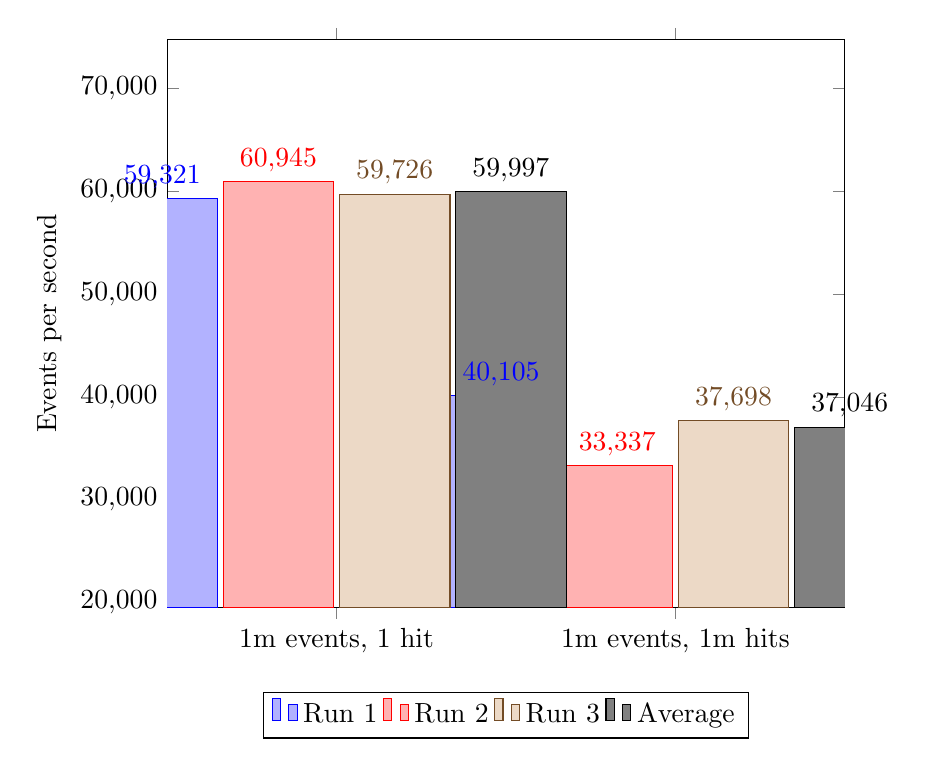
\begin{tikzpicture}
\begin{axis}[
    xtick=data,
	height=250pt,
	ylabel=Events per second,
	enlargelimits=0.5,
	legend style={at={(0.5,-0.15)},
	anchor=north,legend columns=-1},
	ybar,
	bar width=40pt,
	symbolic x coords={{1m events, 1 hit}, {1m events, 1m hits}},
	nodes near coords,
	nodes near coords style={above}
]
\addplot coordinates {({1m events, 1 hit},59321) ({1m events, 1m hits},40105)};
\addplot coordinates {({1m events, 1 hit},60945) ({1m events, 1m hits},33337)};
\addplot coordinates {({1m events, 1 hit},59726) ({1m events, 1m hits},37698)};
\addplot coordinates {({1m events, 1 hit},59997) ({1m events, 1m hits},37046)}; 
\legend{Run 1, Run 2, Run 3, Average}
\end{axis}
\end{tikzpicture}